\documentclass{article}
\usepackage[utf8]{inputenc}
\usepackage{apacite}
\usepackage{graphicx}   
\graphicspath{{figures/}}

\title{Why are we still building AR Piano Teaching Systems? A Review of Augmented Reality Piano Teaching Systems}
\author{Jordan Aiko Deja}
\begin{abstract}

% this abstract might not make any sense anymore 
     Augmented Reality (AR) piano teaching systems …. Many AR piano teaching systems are available for .. while many research prototypes have tried to .. The development of these tools was based on knowledge drawn from fields of computer graphics, ubiquitous and mobile computing, human-computer interaction and cognitive psychology. 
     
\end{abstract}
\date{July 2020}

\begin{document}

\maketitle


\nocite{*}



\section{Introduction}

\section{Background}

\begin{figure}
    \centering
    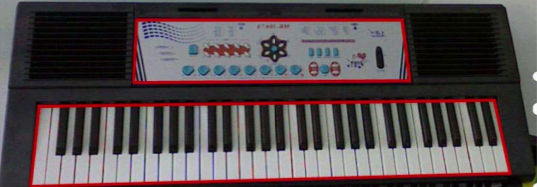
\includegraphics[width=15cm]{figures/pianomarker.png}
    \caption{Piano Augmented Reality marker}
    \label{fig:pianomarker}
\end{figure}



\section{Method}

\begin{figure}
    \centering
    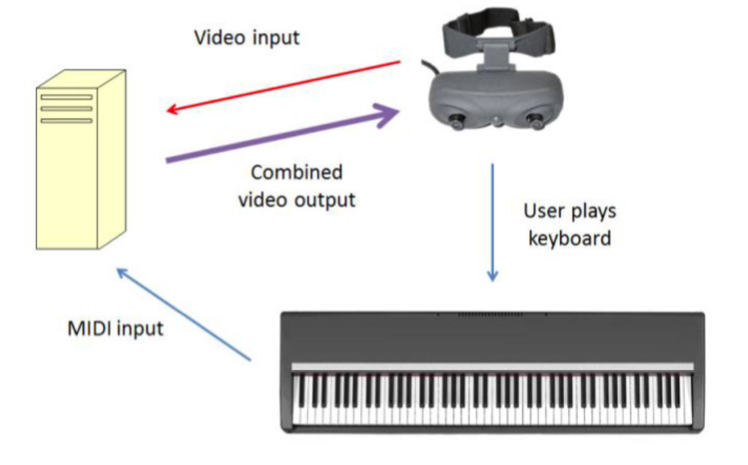
\includegraphics[width=10cm]{figures/headmountedpiano1.png}
    \caption{Architecture of the Head Mounted Piano by cite! }
    \label{fig:pianoheadmountedarch}
\end{figure}

\begin{figure}
    \centering
    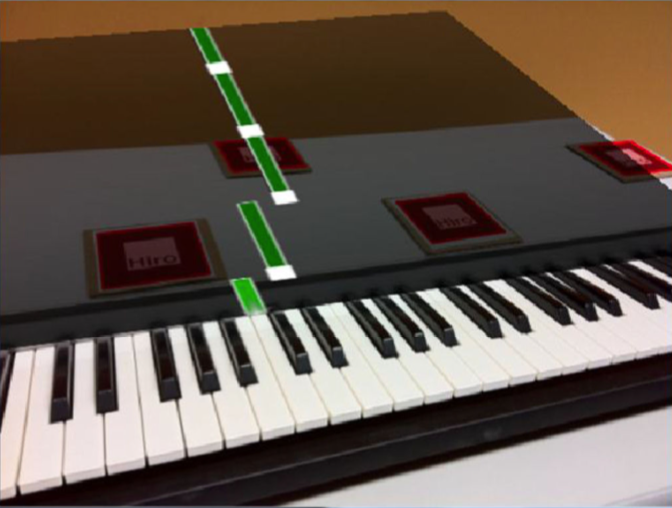
\includegraphics[width=10cm]{figures/headmountedview.png}
    \caption{View from the Head Mounted Piano AR  }
    \label{fig:View from the HeadMounted}
\end{figure}


\section{Affordances of AR piano teaching systems}


\section{Design Strategies of AR piano teaching systems}

\begin{figure}
    \centering
    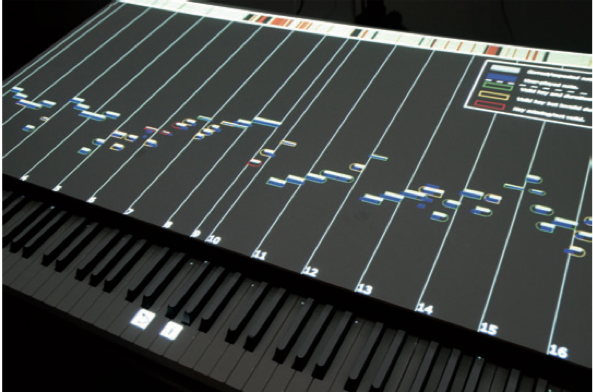
\includegraphics[width=10cm]{figures/piano}
    \caption{View of the Detailed Screen of P.I.A.N.O.› }
    \label{fig:View from the HeadMounted}
\end{figure}



\section{Visualisations}



\section{Agents and Tutors}
\section{Learning Modes}
\section{Evaluation Techniques}
\section{Discussion and Future Directions}

% overview of audio augmented reality
% classical works in audio augmented reality
% visualizations in audio
% audio and lighting effects in performance media
% usability studies involving audio augmented reality
% novel works and audio ar on inclusive music (for def or pwd)




% music features and visualization

% taxonomy of AR and music 

% music decorates space by andre
% using visualization 




\bibliographystyle{apacite}
\bibliography{references}

\end{document}
